\section{Evidence, reproducibility and integration}
\label{sec:evidence}

The deliverable is organized so that a repository reviewer can assess the
mathematical statement, the executable operation, and its source contract
separately.  The article is complete in the accompanying PDF and LaTeX
sources.  The new Python modules are additive research code; the pinned
upstream snapshot is present to make reproduction independent of later
repository changes.

\subsection{Claim and implementation matrix}

\begin{longtable}{@{}P{.27\linewidth}P{.31\linewidth}P{.36\linewidth}@{}}
\toprule
Result & Delivered implementation & Boundary of the claim\\
\midrule
\endfirsthead
\toprule
Result & Delivered implementation & Boundary of the claim\\
\midrule
\endhead
Genus budget and forest quotient & Producer, independent graph checker,
shared source-parent forest & A graph certificate binds incidences and Euler
labels.  Actual ball absorption needs verified geometry and irreducibility.\\
Initial torus admissibility & Geometric source decomposition, independent
raw replay, exact canonical-diagram wrapper & Empty initial pattern and
inherited handle charts.  The intermediate core is not a knotted verdict.\\
Occurrence replay and Fibonacci separation & Counter-based replay,
symbolic-family audit and explicit certificate comparisons & Linear
incidence updates exclude source reconstruction; the size separation
compares the maintained explicit format.\\
Native first returns & Pair and four-field codecs, independent source
checker, complete cyclic assembly, exact gap lengths & Local fibre data
and active words; arbitrary later markings and complete base-frame
transport remain outside the contract.\\
Global inventory lemma & Exhaustive eight-label partition regression and
the native decoder's coverage checks & A complete authenticated weighted
histogram is assumed.  Arithmetic pairs alone do not establish geometry.\\
Unmarked reconstruction & Written constructive theorem and explicit
output-size proof & No reconstruction implementation or fixed marking
transport is delivered.\\
Forest transport circuit & Written algebraic construction & Source
parent paths are implemented; arbitrary group labels and geometric chart
transport are not.\\
Quasipolynomial accounting & Conditional theorem and research questions &
The required complete hierarchy, discovery bounds and pattern-size bounds
are not established by this package.\\
\bottomrule
\end{longtable}

\subsection{Final combined verification}

The final combined run passed all \textbf{30 test methods}, with no failures, errors or skips, in 113.179 seconds. Regina 7.4 was available, so its independent topology controls ran. The exact log is \path{results/validation_log.txt}; the machine-readable environment and result are in \path{results/validation_summary.json}.


The graph tests enumerate all 772 connected labelled simple graphs with
one through five vertices and test three root assignments on each, for
2316 graph/root cases.  They also check 500 seeded random multigraphs,
sharp genus examples, parent routes, loops, parallel edges, disconnected
input rejection, altered forest and root records, and strict integer
typing.  Boolean values and floats equal to integers are not accepted as
integer proof fields.  The additional source-to-kernel test authenticates
all 48 supplied decompositions, passes them through the adapter, and
checks their graph certificates independently.  This test explicitly
preserves the generic, non-recognition status on reducible controls.

The source-handle tests compare the new deletion trace and remaining
handle sets against the maintained reducer on all 48 raw source cases.
They also perform independent tetrahedron and local-vertex relabellings,
exercise the canonical unknot, trefoil and figure-eight diagram sources,
and reject forged source provenance.  The reducible manifolds
$(S^1\times D^2)\#\mathbb{RP}^3$ and
$(S^1\times D^2)\#(S^2\times S^1)$ are central controls: their numerical
cycle signatures pass the generic decomposition checker, but are not
solid tori.  Independent Regina tests and the diagram-source gate keep
the distinction executable.

The native suite compares both new codecs with the complete maintained
cyclic interface on 157 recorded triangulation/normal-vector pairs.
An independent literal edge walk covers 146 of them.  Its 219 positive
gaps and 3420 point gaps test exact length, while the cap-only cases and
whole-circle attachments exercise source geometry that a prism-only
adapter would miss.  Resource caps return an inconclusive operation;
they never turn incomplete work into a partial accepted certificate.
The tests also disable discovery routines during replay, alter source
fingerprints and proof fields, and test JSON round trips for large
integers.  The separate 4140-partition enumeration checks the arithmetic
occupancy lemma without relying on a geometric path promise.

These are finite implementation checks.  The asymptotic claims rest on
the proofs in the article.  The package does not claim formal verification
of Python, statistical representativeness of the fixtures, or complete
testing of unrelated maintained recognition subsystems.

\subsection{What the measurements establish}

All source and native tables retain the individual timing samples in
machine-readable JSON.  There are five measurements per arm and source;
the native comparison has an untimed warmup and alternating forward and
reverse arm order, while the source-handle comparison uses seeded
randomized order.  The graph-only experiment uses seven repetitions after
one warmup.  Measurements were made in a shared execution environment,
with Python 3.12.14 on Linux x86-64.  They are medians of finite samples,
without a claim of hardware isolation or a statistical confidence
interval for a population of knot diagrams.

The new native compiler sometimes improves full discovery and replay
together, and sometimes improves discovery while making replay slower.
Its stronger invariants are exact: one census instead of two, logarithmic
terminal labels, exact additional lengths, and a smaller proved scalar
magnitude for the pair codec.  The new source-handle certificate has an
asymptotic size advantage on its proved family, but extra component-record
overhead can make it larger at small sizes.  The canonical trefoil and the
256-bud trefoil show measured source-operator regressions.  These results
support an opt-in integration and further cost analysis; they do not
support a universal speedup claim.

\begin{figure}[htbp]
\centering
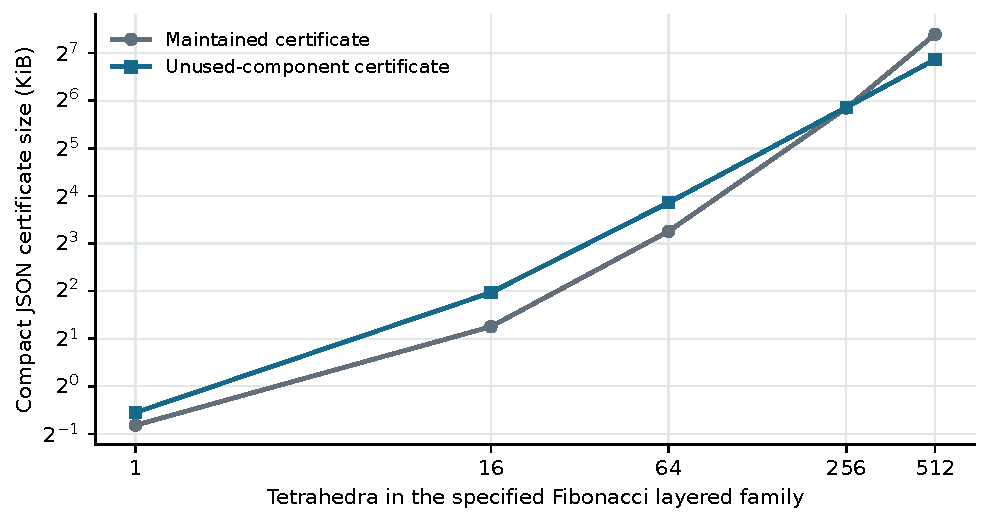
\includegraphics[width=.84\linewidth]{figures/certificate_sizes.pdf}
\caption{Recorded compact-JSON certificate sizes on the specified
Fibonacci layered family.  Lines connect measured points only.  Small
instances expose the new format's overhead; the proof of its asymptotic
advantage is Proposition~\ref{prop:unused-fibonacci-separation}, not a
fit to this plot.}
\label{fig:certificate-sizes}
\end{figure}

The graph experiment isolates the cost of retaining source provenance
while shrinking the operational graph.  Its realizable examples contain
three solid-torus-type vertices and an increasingly long chain of ball-type
vertices.  The kernel always has three vertices and two edges; the
certificate retains the full source-parent forest.

\begin{table}[htbp]
\centering\small
\begin{tabular}{rrrrr}
\toprule
Source vertices & Kernel vertices/edges & Production, ms & Replay, ms & Proof bytes\\
\midrule
10 & 3/2 & 0.034 & 0.044 & 593\\
100 & 3/2 & 0.252 & 0.335 & 2531\\
1000 & 3/2 & 3.003 & 3.499 & 26879\\
10000 & 3/2 & 36.015 & 44.774 & 319877\\
\bottomrule
\end{tabular}
\caption{Graph-only genus-three kernels with full source provenance, seven repetitions. Geometric source authentication and disc-chart construction are excluded.}
\label{tab:attachment-kernel-times}
\end{table}


This experiment excludes construction or authentication of the vertex
manifolds and their disc charts.  It measures the graph routine described
in its theorem, not a hidden geometric ball-recognition algorithm.

\subsection{Package layout and replay}

The principal executable interfaces are as follows.

\begin{description}[style=nextline]
\item[\code{decompose\_unused\_handles}]
Consumes a validated raw torus-boundary source.  Returns a geometric
decomposition and a numerical case, with no irreducibility assertion.
\code{verify\_unused\_handle\_certificate} reconstructs source cells and
replays the trace independently.
\item[\code{compile\_diagram\_initial\_core}]
Consumes a classical knot diagram and derives its canonical exterior.
Its checked outputs are \code{UNKNOT}, \code{ADMISSIBLE\_CORE}, or
resource-limited \code{INCONCLUSIVE}.  The independent wrapper checks
the exact diagram and exterior provenance before using the genus theorem.
\item[\code{kernel\_from\_decomposition}]
Converts the source decomposition format into a rooted-forest graph
certificate.  It is an adapter, not a substitute for the geometric
checker.  The independent graph checker accepts the original Euler labels
and edge incidences alongside the proposed certificate.
\item[\code{normal\_parallelity\_moment\_words}]
Consumes a triangulation and binary normal coordinates, and returns the
complete native cyclic interface with exact lengths.  The independent
checker rebuilds the source through the reference path.  The optional
\code{moments\_from\_parallelity\_packet} entry point additionally verifies
and retains a complete upstream parallelity certificate.
\end{description}

From the archive root, the following commands run the complete delivered
suite and small verified examples:
\begin{lstlisting}[language=bash]
python3 -m pip install -r requirements.txt
python3 run_checks.py
python3 examples.py
\end{lstlisting}
The test runner inserts the new code and pinned native snapshot into its
import path.  The examples show a positive unknot certificate, the
intermediate trefoil core, and an exact native boundary query.  Representative
native certificates can also be replayed without running discovery, using
\code{code/native\_moments\_replay.py} with the import path documented
in the root README.

The new algorithms use Python's standard library.  Regina 7.4 is listed
to reproduce the separate topology controls in the complete recorded run.
Matplotlib is needed only to regenerate the figures, which are already
included.  A TeX distribution builds the article using
\code{latexmk -pdf hierarchy\_primitives.tex} from its article directory.
No private external data source is needed for reproduction.

\subsection{Suggested repository integration}

The initial integration should preserve the package as an additive
research contribution, with its exact source revision and evidence.
\code{integration/INTEGRATION.md} maps the modules to a proposed maintained
placement and records the private source APIs they currently use.
The pinned source snapshot is for reproduction; an integrated tree should
use the repository's matching maintained modules instead of maintaining a
second copy of them.

For a first opt-in recognizer change, call the canonical-diagram initial
compiler at the same stage as the existing source-handle operator.
Accept a positive result only through the diagram-bound checker.  A
returned core should enter the next stage only once that stage supports
the inherited handle presentation and its normal-coordinate interface.
For the boundary compiler, compare full old and new outputs in a
differential integration mode, then select the new operator only under
its documented source contract.  Preserve caps and interruption behavior.

No default dispatch or remote repository mutation is included in this
deliverable.  The package supplies concrete code and proofs for review;
the unresolved patterned and global interfaces remain explicit research
tasks.  The goal of the proposed integration is to reduce real local work
while keeping every eventual recognition claim attached to its geometric
authority and complete complexity accounting.
